\section{The derivation of the noise spectrum from the cavity} 
\label{sec:cavitynoise}

The Hamiltonian of a single-mode cavity is
\begin{equation}
\label{eq:cavity_Hamiltonian}
    H = \hbar \omega_{\rm c}(C^{\dagger}C+\frac{1}{2}),
\end{equation}
where $\omega_{\rm c}/2\pi$ is the cavity resonant frequency and $C$ is the 
annihilation operator of the inner cavity field. The cavity field is coupled 
to the modes $A$ of a transmission line with the rate $\kappa_2$. The cavity 
field is also coupled to the environment modes $B$ with the rate $\kappa_0$. 
Based on the model of Fig.~\ref{fig:cavity_in_out.jpg} and the input-output 
theory, the equation of motion for $C$ is obtained:
\begin{equation}
\label{eq:EOM}
    \frac{dC}{dt} = -i\omega_{\rm c} C - \frac{\kappa_2+\kappa_0}{2} C + \sqrt{\kappa_2} A_{\rm in} + \sqrt{\kappa_0}B_{\rm in}.
\end{equation}
A boundary condition holds for the transmission modes:
\begin{equation}
\label{eq:BC}
    A_{\rm out} = \sqrt{\kappa_2} C - A_{\rm in}.
\end{equation}
Considering working in a rotating frame of the signal frequency $\omega$ near 
$\omega_{\rm c}$, the equation of motion becomes:
\begin{equation}
\label{eq:EOM_rotating_frame}
    -i\omega C + \frac{dC}{dt} = -i \omega_{\rm c} C - \frac{\kappa_2+\kappa_0}{2} C + \sqrt{\kappa_2} A_{\rm in} + \sqrt{\kappa_0} B_{\rm in}.
\end{equation}
The steady state solution for the cavity field is: 
\begin{equation}
\label{eq:cavity_field}
    C = \frac {\sqrt{\kappa_2} A_{\rm in} + \sqrt{\kappa_0} B_{\rm in}} {-i (\omega-\omega_{\rm c}) + \frac{\kappa_2+\kappa_0}{2} }.
\end{equation}
By substituting Eq.~\eqref{eq:cavity_field} into Eq.~\eqref{eq:BC}, the 
reflected modes of the transmission line $A_{\rm out}$ are expressed in terms 
of the input modes of the transmission line $A_{\rm in}$ and the environment 
$B_{\rm in}$:
\begin{equation} \label{eq:output_field}
\begin{split}
	 A_{\rm out} & =  \frac{i(\omega - \omega_{\rm c}) + \frac{\kappa_2-\kappa_0}{2}}{-i(\omega - \omega_{\rm c}) + \frac{\kappa_2+\kappa_0}{2}} A_{\rm in} + \frac{\sqrt{\kappa_2 \kappa_0}}{-i(\omega - \omega_{\rm c}) + \frac{\kappa_2+\kappa_0}{2}} B_{\rm in} \\
                           & = \frac{-(\omega-\omega_{\rm c})^2 + \frac{\kappa_2^2-\kappa_0^2}{4}+i\kappa_2(\omega-\omega_{\rm c})}{(\omega-\omega_{\rm c})^2+(\frac{\kappa_2+\kappa_0}{2})^2} A_{\rm in} + \frac{\sqrt{\kappa_2\kappa_0}\frac{\kappa_2+\kappa_0}{2}+i\sqrt{\kappa_2\kappa_0}(\omega-\omega_{\rm c})}{(\omega-\omega_{\rm c})^2+(\frac{\kappa_2+\kappa_0}{2})^2} B_{\rm in}.
\end{split}
\end{equation}

Therefore, the autocorrelation of $A_{\rm out}$ is related to those of $A_{\rm in}$ and $B_{\rm in}$:
\begin{equation}
\label{eq:autocorrelation}
\begin{split}
    \langle A_{\rm out}^\dagger A_{\rm out} \rangle  = & \frac{[(\omega-\omega_{\rm c})^2 - \frac{\kappa_2^2-\kappa_0^2}{4}]^2+\kappa_2^2(\omega-\omega_{\rm c})^2}{[(\omega-\omega_{\rm c})^2+(\frac{\kappa_2+\kappa_0}{2})^2]^2} \langle A_{\rm in}^\dagger A_{\rm in} \rangle \\ & +  \frac{\kappa_2\kappa_0(\frac{\kappa_2+\kappa_0}{2})^2+\kappa_2\kappa_0(\omega-\omega_{\rm c})^2}{[(\omega-\omega_{\rm c})^2+(\frac{\kappa_2+\kappa_0}{2})^2]^2}\langle B_{\rm in}^\dagger B_{\rm in} \rangle.
\end{split}
\end{equation}
The spectrum from the cavity $S(\omega)$ is found to be related to the spectrum 
of the readout transmission line $S_{\rm rt}(\omega)$ and the spectrum of the 
cavity environment $S_{\rm cav}(\omega)$:
\begin{equation}
\label{eq:spectrum_relation}
\begin{split}
    S(\omega) & = \frac{[(\omega-\omega_{\rm c})^2 - \frac{\kappa_2^2-\kappa_0^2}{4}]^2+\kappa_2^2(\omega-\omega_{\rm c})^2}{[(\omega-\omega_{\rm c})^2+(\frac{\kappa_2+\kappa_0}{2})^2]^2} S_{\rm rt}(\omega) \\ & + \frac{\kappa_2\kappa_0(\frac{\kappa_2+\kappa_0}{2})^2+\kappa_2\kappa_0(\omega-\omega_{\rm c})^2}{[(\omega-\omega_{\rm c})^2+(\frac{\kappa_2+\kappa_0}{2})^2]^2}S_{\rm cav}(\omega).
\end{split}
\end{equation}
As the the readout transmission line and the cavity environment are both in 
thermal states, i.e. $S_{\rm rt}(\omega)=\left[n_{\rm BE}(T_{\rm rt})+1/2\right]\hbar\omega$ 
and $S_{\rm cav}(\omega)=\left[n_{\rm BE}(T_{\rm cav})+1/2\right]\hbar\omega$, where 
$n_{\rm BE}$ is the mean photon number given by the Bose-Einstein distribution, 
$S(\omega)$ is white if $T_{\rm cav}=T_{\rm rt}$, and Lorentzian if 
$T_{\rm cav} \gg T_{\rm rt}$.

\begin{figure}[htbp]
    \centering
    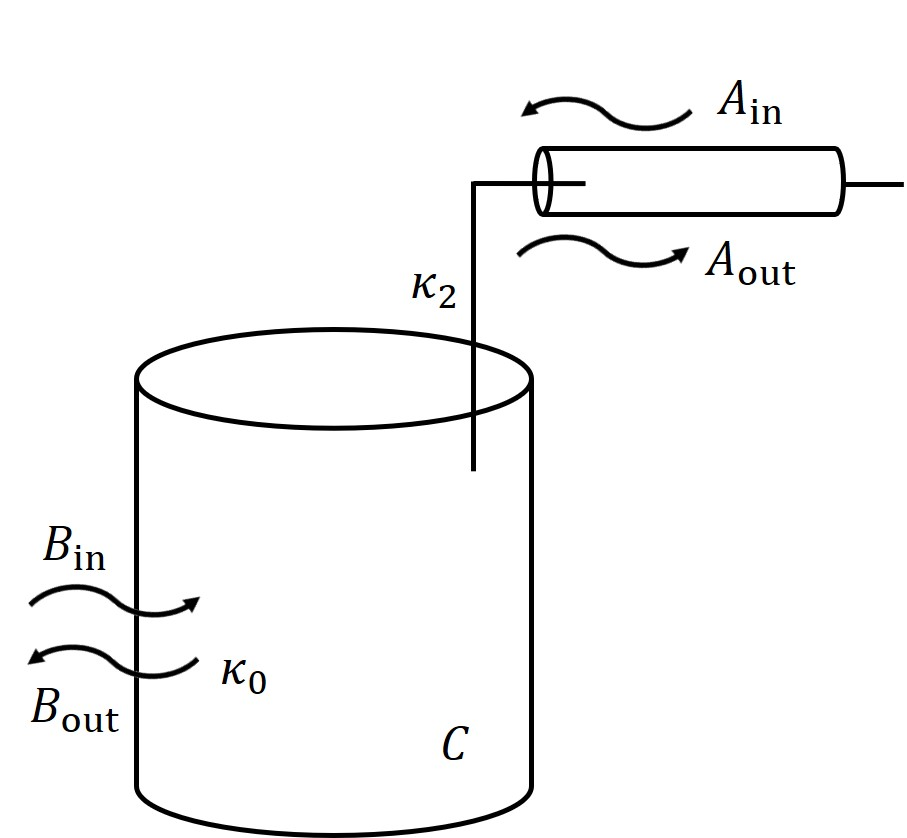
\includegraphics[width=8.6cm]{figures/cavity_in_out.jpg}
    \caption{A cavity is coupled to the modes of transmission line $A$ with the 
rate $\kappa_2$ and the modes of environment $B$ with the rate $\kappa_0$.}
    \label{fig:cavity_in_out.jpg}
\end{figure}


